\textbf{Griva, Nash, Sofer 2.2.3}

Consider the problem

\begin{align*}
  \text{minimize}   \qquad & f(x) = x_1 \\
  \text{subject to} \qquad & x_1^2 + x_2^2 \le 4 \\
                    \qquad & x_1^2 \ge 1
\end{align*}

Graph the feasible set and identify any local or global minimizers.

\begin{solution}
  We plot the feasible set below:

  \begin{figure}[h]
    \centering
    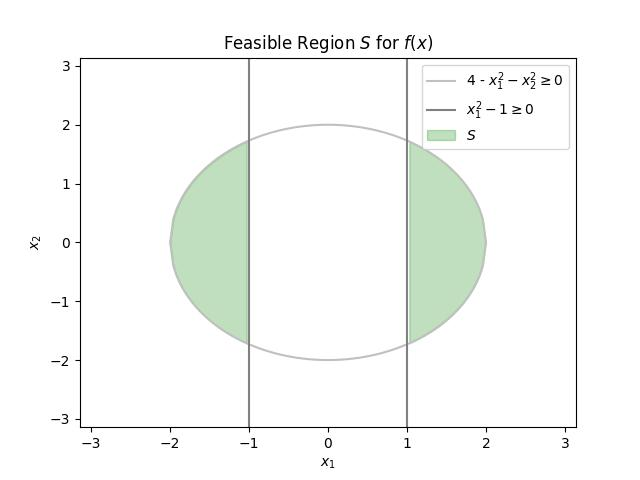
\includegraphics[width=\textwidth]{problem_2.jpg}
    \caption{Feasible region $S$ (green)}
  \end{figure}

  From the above plot, we see that no global minima of the objective function exist in the feasible region $S$.\footnote{
    In fact, since the domain of $f$ is all of $\mathbb{R}$ and $f$ is strictly decreasing, no global minimum of $f$ exists at all.
  } 
  A local minimum does exist at $x = (1, 1)$ which takes the value $f(x) = x_1 = 1$.
  \ \\
\end{solution}